\chapter{Background}
\label{background}
\rhead{}
\lhead{Background}

In questo primo capitolo verranno esposti ed analizzati, nelle parti che interessano lo stage, gli ultimi studi effettuati all'interno del gruppo di ricerca con cui ho lavorato in ambito di offuscamento dei dati e automazione dei test in ambiente Android. In particolare modo verranno presentati ad alto livello ed esaminati brevemente gli strumenti di potenziale interesse già realizzati in questi studi con il fine di valutarne un possibile riutilizzo. L'analisi  includerà inoltre l'identificazione di possibili limitazioni e criticità  delle soluzioni adottate. %L'obiettivo generale di questo capitolo consiste quindi nel dare un'idea complessiva della base  sul punto di partenza dello stage.
%e l'analisi effettuata, in alcuni suoi punti, potrebbe non risultare completamente chiara fino alla lettura del capitolo successivo.

\subsection*{Studi di riferimento}
\begin{itemize}[nosep]
\item \textbf{Belisario A.} (2016/2017) \textcolor{gray}{Tesi magistrale}
\newline \emph{Analisi empirica dell'influenza delle tecniche di offuscamento dei dati sulla riproduzione dei fallimenti del software.} 

\item  \textbf{Triolo D.} (2016/2017)  \textcolor{gray}{Relazione triennale}
\newline \emph{Test app Android con dati offuscati: setup ambiente di test e valutazione empirica dei fallimenti del software.}

\item  \textbf{Mendieta A.} (2016/2017)   \textcolor{gray}{Relazione triennale}
\newline \emph{Realizzazione di uno strumento per l’esecuzione automatica di test parametrici in Android.}

\item  \textbf{Sormani D.} (2019/2020) \textcolor{gray}{Relazione triennale}
\newline \emph{Analisi empirica dell’impatto di tecniche di offuscamento di dati sulla riproducibilità di bug.}
\end{itemize}
\newpage
\section{Soluzioni candidate al riutilizzo}
\rhead{Soluzioni candidate al riutilizzo}
\noindent Per il raggiungimento di alcuni sotto-obiettivi dello stage, è stato valutato un possibile riutilizzo delle seguenti soluzioni realizzate negli studi precedenti:
\bigskip
\begin{itemize}[nosep]

\item[]\textbf{\emph{Ob.1} Offuscamento dei dati} \

\begin{itemize}[nosep]
\item[] \ul{Obiettivo}  Realizzazione di un componente in grado di applicare le tecniche di offuscamento e restituire le tuple offuscate.
\item[]  \ul{Soluzione}  Libreria di offuscamento + LoadDataPool
\end{itemize}

%\smallskip
%\item[]\textbf{Ob.2 Creazione del caso di test}
%\begin{itemize}[nosep]
%\item[] \ul{Obiettivo}  Ricerca della migliore soluzione per la registrazione e parametrizzazione del caso di test che genera il bug.
%\item[]  \ul{Soluzione}  Parametrizzazione con JUnitParams + Registrazione con Espresso Test Recorder
%\end{itemize}

\smallskip
\item[]\textbf{\emph{Ob.3} Automazione dell'esecuzione di test parametrici in ambiente Android}
\begin{itemize}[nosep]
\item[] \ul{Obiettivo}  Realizzazione di un componente in grado di eseguire automaticamente instrumented tests parametrici e capace di catturarne il risultato. 
\item[]  \ul{Soluzione}  AndroidApp tool
\end{itemize}
\end{itemize}
\bigskip
\noindent Tutte le soluzioni elencate (Libreria di offuscamento, LoadDataPool, AndroidAppTool) vengono analizzate e valutate singolarmente nei capitoli successivi (Sezione \ref{liboff}, Sezione \ref{loaddatapool}, Sezione \ref{androidapptool}) . 

\section{Libreria di offuscamento}
\rhead{Libreria di offuscamento}
\label{liboff}
La libreria di di offuscamento considerata è stata sviluppata nella tesi magistrale “Analisi empirica dell'influenza delle tecniche di offuscamento dei dati sulla riproduzione dei fallimenti del software” del collega Andrea Belisario. La libreria  \textbf{offre la possibilità di ottenere, dato un input appartenente ad un certo dominio, un output modificato  secondo una particolare tecnica di offuscamento}.
%Uno tra i sotto-obiettivi che si vogliono raggiungere include la realizzazione di un componente in grado di applicare le tecniche di offuscamento e restituire le tuple offuscate. Nella tesi magistrale “Analisi empirica dell'influenza delle tecniche di offuscamento dei dati sulla riproduzione dei fallimenti del software” del collega Andrea Belisario, è stata sviluppata una libreria che \textbf{offre la possibilità di ottenere,  dato un input appartenente a un certo dominio,  un output modificato secondo una particolare tecnica di offuscamento}. 

%%VALUTAZIONE
%Per le finalità dello stage la libreria non ha bisogno di modifiche e risulta utile riutilizzarla nella sua interezza.

\subsection{Dettagli progettuali e implementativi}
Nel contesto in cui è stata sviluppata la libreria, è essenziale che il dominio dei dati offuscati (output) sia coerente con il dominio dei dati non offuscati (input). Si può facilmente intuire, per esempio, l'impossibilità di eseguire test che ammette solo numeri avendo a disposizione solo stringhe. Per questo motivo la libreria è stata progettata in modo tale che ogni tecnica di offuscamento offra due metodi:
\begin{itemize}[nosep]
\item [$\blacksquare$] \textbf{offuscaDato(dato) = datoOffuscato} \newline
Il metodo va ad offuscare il dato in input "dato" e restituisce un valore che potrebbe non essere coerente con il suo dominio, ma che rispetta la definizione della tecnica di offuscamento di turno.
\item [$\blacksquare$] \textbf{rendiDominioCoerente(datoOffuscato)} \newline
Il metodo prende in input il risultato del metodo precedente e restituisce un valore coerente con il dominio dell’attributo offuscato, che sia quindi utilizzabile per i test.
\end{itemize}
\bigskip
\noindent La coerenza dei domini richiesta dalla libreria, ottenuta tramite l'applicazione dei metodi sopra illustrati, implica l'utilizzo di una logica che gestisca le varie \textbf{tipologie di dato}. La logica è stata implementata con la realizzazione di una classe astratta dalla quale ereditano tutte le tipologie di dato previste dalla libreria:
\begin{itemize}[nosep]
\item [$\blacksquare$] \textbf{Categorici} (Categorical) \newline
I valori categorici possono assumere solamente un numero finito di valori. In ambito informatico l’equivalente dei valori categorici è rappresentato dai tipi enumerativi.
\item [$\blacksquare$] \textbf{Continui} (Continuos)\newline
I valori continui possono assumere un numero non finito di valori all’interno di un range. 
\item [$\blacksquare$] \textbf{Stringhe} (StringType)\newline
I valori che non possono essere definiti come 'Categorici' o 'Continui', nel dominio informatico, possono essere rappresentati mediante stringhe.
\end{itemize}


\subsection{Tecniche di offuscamento}
La libreria realizzata racchiude le tecniche di offuscamento più utilizzate e rivisitate dal collega per essere adattate al meglio alle esigenze dello studio. Le tecniche incluse possono essere \emph{perturbative}, quando il dato viene sostituito e alcuni dettagli vengono rimossi, oppure  \emph{non perturbative}, quando il dato originale non viene alterato, ma vengono soppresse alcune informazioni.

\subsection*{Tecniche non perturbative}

\noindent\textbf{Local Suppression}
\begin{adjustwidth}{2.5em}{0pt}
 \textbf{\textcolor{gray}{Definizione}} \newline
Data una tupla T, la nuova tupla T’ contiene tutti gli attributi contenuti in T con i valori di alcuni attributi soppressi. \newline
\textbf{\textcolor{gray}{Rivisitazione}} \newline
Ai fini della libreria, non ha utilità inserire valore NULL (soppressione) in quanto si otterrebbero sempre le stesse risposte in qualunque esecuzione del test. La soluzione adottata prevede la sostituzione dei valori da offuscare con valori generati randomaticamente nel loro dominio.
\end{adjustwidth}
\medskip
\noindent\textbf{Global Recoding}
\begin{adjustwidth}{2.5em}{0pt}
 \textbf{\textcolor{gray}{Definizione}} \newline
Può essere utilizzata solo sui tipi di valori continui. Il dominio di un attributo viene	suddiviso in N intervalli disgiunti non necessariamente della stessa dimensione, ad ognuno dei quali viene assegnata un’etichetta. Data una tupla T, i valori degli attributi contenuti in T’ saranno sostituiti dalle etichette degli intervalli a cui appartengono. \newline
\textbf{\textcolor{gray}{Rivisitazione}} \newline
Ai fini della libreria, non ha senso sostituire il valore di un dato con l’etichetta dell'intervallo a cui appartiene (inoltre la coerenza del dominio non sarebbe rispettata). In questo caso viene generato un valore random all’interno dell’intervallo in cui si trova il dato originale. 
\end{adjustwidth}
\medskip
\noindent\textbf{Top/Bottom Coding}
\begin{adjustwidth}{2.5em}{0pt}
 \textbf{\textcolor{gray}{Definizione}} \newline
Può essere utilizzata solo sui tipi di valori continui. A partire dai valori presenti in una tabella T viene definito un limite top o bottom, che indicano rispettivamente il limite superiore e il limite inferiore nel dominio di un valore continuo. I campioni per i quali l’attributo da offuscare supera, o è inferiore, al valore di soglia, vengono sostituiti con l’etichetta '$>$ TL', se si tratta di un limite superiore o '$<$ BL', se si tratta di un limite inferiore. \newline
\textbf{\textcolor{gray}{Rivisitazione}} \newline
Ai fini della libreria, non ha senso sostituire il valore di un dato con un’etichetta (inoltre la coerenza del dominio non sarebbe rispettata). In questo caso viene generato un valore random inferiore o maggiore alla soglia.
\end{adjustwidth}
\medskip
\noindent\textbf{Generalizzazione}
\begin{adjustwidth}{2.5em}{0pt}
 \textbf{\textcolor{gray}{Definizione}} \newline
Può essere applicata sia a valori continui che categorici. La tecnica prevede di sostituire il valore di un attributo con un suo rappresentante gerarchico superiore.  Le gerarchie possono essere rappresentate mediante gli alberi: nella radice dell’albero si trova il valore più generico mentre le foglie rappresentano i valori più specifici. Il valore offuscato sarà un antenato del valore stesso.\newline
\textbf{\textcolor{gray}{Rivisitazione}} \newline
Nessuna rivisitazione.
\end{adjustwidth}

\subsection*{Tecniche perturbative}

\noindent\textbf{PRAM}
\begin{adjustwidth}{2.5em}{0pt}
 \textbf{\textcolor{gray}{Definizione}} \newline
La tecnica PRAM prevede di sostituire il valore categorico della tupla con un altro valore categorico adottando la tecnica della probabilità. Il risultato è l'introduzione di volontari errori nella classificazione dei dati raccolti, in modo che non sia possibile risalire all’identità del proprietario. Per l’utilizzo di questa tecnica viene creata la matrice Markoviana, una matrice di transizione contenente le probabilità di passare da uno stato ad un altro, nel nostro caso di osservare un valore categorico in corrispondenza del valore da offuscare. \newline
\textbf{\textcolor{gray}{Rivisitazione}} \newline
Nessuna rivisitazione.
\end{adjustwidth}
\medskip
\noindent\textbf{Rounding}
\begin{adjustwidth}{2.5em}{0pt}
 \textbf{\textcolor{gray}{Definizione}} \newline
La tecnica rounding opera in maniera analoga rispetto alla tecnica Global Recoding separando il dominio del valore in N intervalli e calcolando per ognuno di questi il rounding point, che solitamente è il valore medio di ogni intervallo.  Il valore viene quindi offuscato sostituendolo con il rounding point dell’intervallo a cui il valore appartiene.\newline
\textbf{\textcolor{gray}{Rivisitazione}} \newline
Ai fini della libreria, ha senso utilizzare sempre come rounding point il valore medio dell'intervallo. 
\end{adjustwidth}

\subsection{Valutazione della soluzione}
Per le finalità dello stage la libreria non ha bisogno di modifiche e risulta utile riutilizzarla nella sua interezza.
%\section{Tool orchestratore}
%Il raggiungimento della maggio parte dei sotto-obiettivi identificati nella sezione 'Obiettivo dello stage' dell'Introduzione,  implica la realizzazione di un tool orchestratore in grado di gestire l'intero processo.  Gli studi effettuati precedentemente dai colleghi hanno portato allo sviluppo di alcuni strumenti in grado di adempire ad alcuni dei requisiti, in particolar modo:

\newpage

\section{LoadDataPool}
\rhead{LoadDataPool}
\label{loaddatapool}
LoadDataPoll è il componente principale dell'architettura dello strumento realizzato da A. Belisario nella tesi magistrale "Analisi empirica dell’influenza delle tecniche di offuscamento dei dati sulla riproduzione dei fallimenti del software". Il tool è in grado di riprodurre automaticamente test per applicazioni desktop utilizzando come parametri dati precedentemente offuscati con le tecniche della libreria trattata nella sezione precedente (Sezione \ref{liboff}).
\subsection{Architettura della soluzione}
 \begin{figure}[H]
	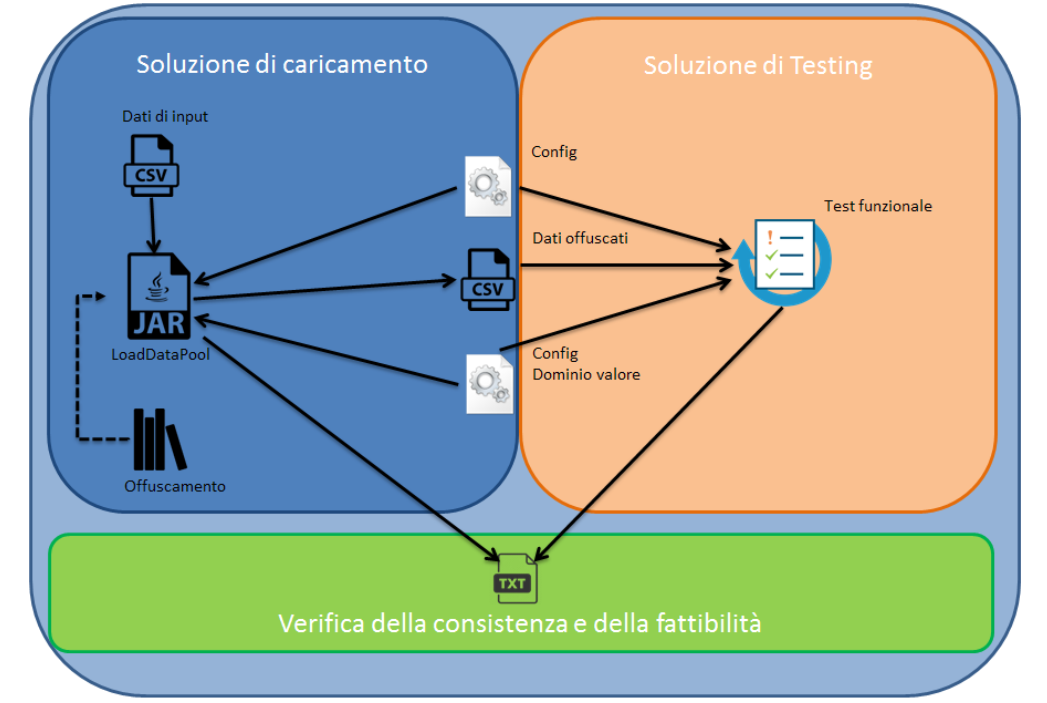
\includegraphics[scale=0.46]{architettura.della.soluzione.belisario}
	\centering
	\caption[]{Architettura della soluzione \footnotemark }
    \label{fig:arch1}
\end{figure}
\footnotetext{Immagine realizzata da A. Belisario}
\noindent Come illustrato nella Figura \ref{fig:arch1}, l'architettura della soluzione si compone di 3 parti:
\begin{itemize} [nosep]
\item \textbf{Modulo di caricamento} \newline
Il modulo di caricamento si occupa di:
\begin{itemize} [nosep]
\item  leggere le tuple in input da un file csv; 
\item leggere le informazioni necessarie all'offuscamento da dei file xml di configurazione ;
\item offuscare i dati in input in base alle informazioni lette (come tecnica di offuscamento e dominio dei dati).
 \end{itemize}
Il modulo produce in output un file csv contenente le tuple offuscate. Il file prodotto sarà uno dei file in input per il modulo di testing.
\item  \textbf{Modulo di testing} \newline
Il modulo di testing si preoccupa di lanciare in maniera automatica un test per ogni tupla del file ricevuto dal modulo di caricamento e di catturarne il risultato. 
\item  \textbf{Modulo di verifica} \newline
Il modulo di verifica valuta l'efficacia dell'offuscamento (se è o non è in grado di riprodurre il bug) e si occupa della creazione di un file di log in output.
\end{itemize}

\subsection{Valutazione della soluzione}
Per le finalità del sotto-obiettivo considerato risulta utile riutilizzare solo il modulo di caricamento (che si occupa di orchestrare l'offuscamento), in quanto comunque la parte di automazione dei test è stata realizzata ad hoc per applicativi desktop  e non potrebbe essere in nessun modo riutilizzata in ambiente Android.  Il riutilizzo di parte di questo componente implica il dover adottare la stessa architettura prevista da A. Belisario, che prevede in input due file di configurazione distinti: uno per il dominio e uno per le tecniche di offuscamento. 

\section{AndroidApp tool}
\rhead{AndroidApp tool}
\label{androidapptool}
Un altro dei sotto-obiettivi che si vogliono raggiungere include la realizzazione di un componente in grado di eseguire automaticamente instrumented tests parametrici su applicazioni Android e capace di catturarne il risultato. A questo sotto-obiettivo è in realta fortemente legata anche la ricerca di una soluzione per la registrazione e parametrizzazione del caso di test che genera il bug (\emph{Ob.2}).  Nella relazione “Realizzazione di uno strumento per l’esecuzione automatica di test parametrici in Android” del collega Anthony Mendieta, viene esposto e realizzato uno strumento, chiamato AndroidApp tool, che risponde quasi in toto ai requisiti del sotto-obiettivo. 
\subsection{Architettura della soluzione}
 \begin{figure}[H]
	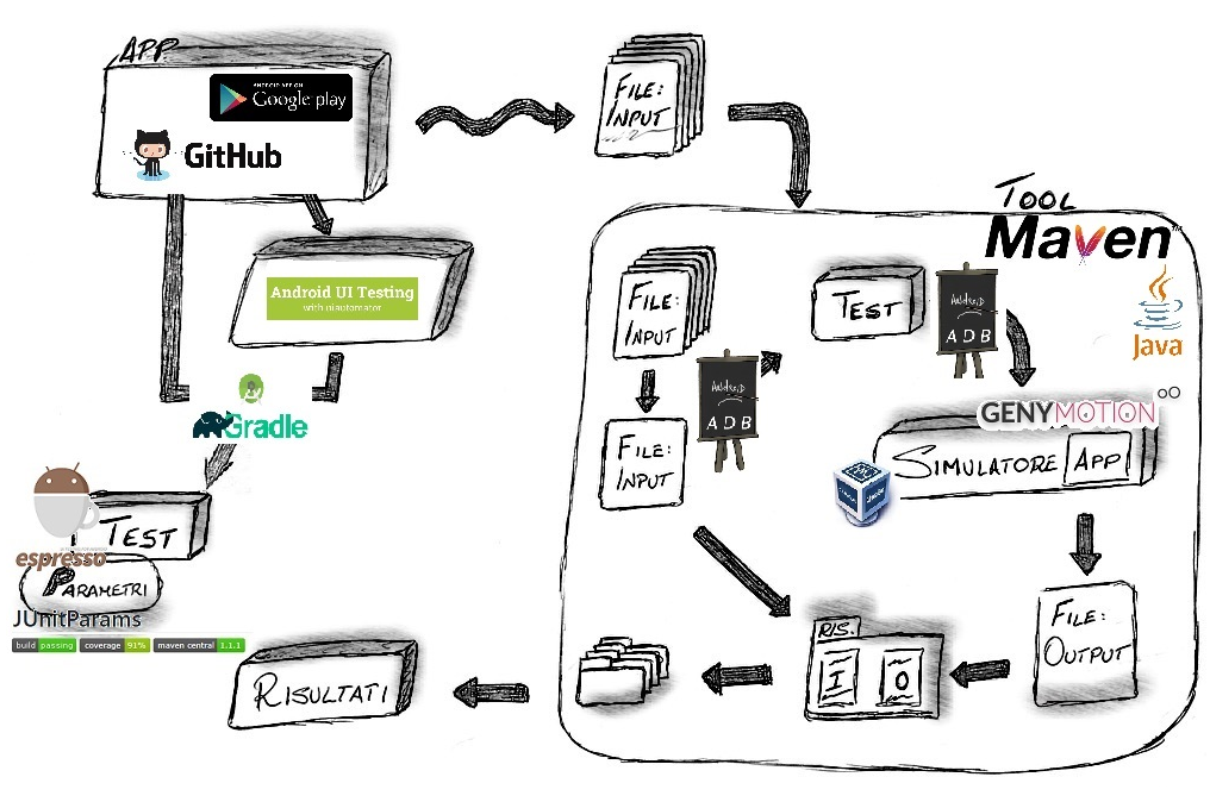
\includegraphics[scale=0.35]{architettura.android.app.tool}
	\centering
	\caption[]{Architettura della soluzione \footnotemark }%\footnote{Immagine realizzata da A. Belisario}
    \label{fig:arch.mendieta}
\end{figure}
\footnotetext{Immagine realizzata da A. Mendieta}

\noindent L'\textbf{architettura della soluzione} realizzata dal collega, illustrata in Figura \ref{fig:arch.mendieta}, prevede in input:
\begin{itemize} [nosep]
\item \textbf{file di input} \newline
Il file di input è un file txt che contiene i  parametri con cui eseguire i test, separati da una virgola. Il documento può essere formato da più righe, ognuna delle quali corrisponde ai parametri di esecuzione di un singolo test.
\item   \textbf{APK dell'applicazione} \newline
L' APK dell'applicazione che si vuole testare.
\item  \textbf{APK di test} \newline
L'APK di test dell'applicazione che si vuole testare contenente la classe di test parametrica.
\item  \textbf{file di configurazione} \newline
File di configurazione utile al funzionamento del tool.
\end{itemize}
\bigskip
\noindent Il \textbf{flusso di normale funzionamento} del tool può essere sintetizzato come segue:
\begin{enumerate} [nosep]
\item Lettura del file di configurazione
\item Installazione dell'APK dell'applicazione e dell'APK di test sull'emulatore (se prevista dal file di configurazione)
\item Lettura del file di input
\item Per ogni riga letta dal file di input
\begin{itemize} [nosep]
\item [1] Creazione di un file contenente la singola riga letta
\item [2] Push del file creato nel punto precedente sull'emulatore (nel percorso interno specificato nel file di configurazione)
\item [3]  Lancio della classe di test parametrica (utilizza come parametri i valori contenuti nel file caricato sull'emulatore nel  punto precedente)
\item [4]  Cattura del risultato del test in un file di testo  (in caso di errore salva il log in un file di testo a parte)
\end{itemize}
\end{enumerate}

\subsubsection{File di configurazione}
La soluzione proposta prevede la presenza di un file di configurazione in cui devono essere specificati i seguenti parametri:
\begin{itemize} [nosep]
\item[]\textbf{PathAPK} \newline
Indirizzo interno del pacchetto in cui si trova l'APK dell'applicazione
\item []\textbf{PathAPKTest} \newline
Indirizzo interno del pacchetto in cui si trova l'APK di test dell'applicazione
\item[] \textbf{PathOutput} \newline
Indirizzo interno del pacchetto in cui creare i file prodotti dal tool
\item[] \textbf{PathInput} \newline
Indirizzo interno del pacchetto in cui si trovano i file di input
\item[] \textbf{PathIntoAndroid} \newline
Indirizzo interno del device in cui si trova la cartella riservata all’applicazione da testare, nella quale verranno copiati i file di input da testare
\item []\textbf{dirClassTest} \newline
Nome del pacchetto all’interno del quale si trova la classe di test
\item[] \textbf{dirRunWith} \newline
Indirizzo completo della strumentazione che si occuperà del lancio della
classe di test 
\item []\textbf{installAPK} \newline
Valore booleano che indica se si deve procedere con l’istallazione
o la reinstallazione dell’APK sul device
\item[] \textbf{installAPKTest} \newline
Valore booleano che indica se si deve procedere con l’istallazione
o la reinstallazione dell’APK di test sul device
\item[] \textbf{eseguireTest} \newline
Valore booleano che indica se si deve procedere con il lancio dei test parametrici
\end{itemize}


\subsubsection{Creazione della classe di test}
Nella soluzione vengono proposte due modalità per la creazione della classe di test:
\begin{itemize} [nosep]
\item \textbf{Scrittura a mano del caso di test} \newline
Modalità obbligatoria quando non si ha a disposizione il codice sorgente. In questo caso è fondamentale l'utilizzo di UI Automator Viewer(Appendice A - UI Automator Viewer).
\item \textbf{Registrazione del caso di test} \newline
Modalità utilizzabile solo quando si è in possesso del codice sorgente. Per la registrazione del caso di test viene utilizzato Espresso Test Recorder(Appendice A - Registrazione del caso di test con Espresso Test Recorder).
\end{itemize}

\subsubsection{Parametrizzazione del caso di test}
Per la parametrizzazione del caso di test viene utilizzata la libreria JUnitParams, che è in grado di di leggere automaticamente i parametri da un file nel device. La libreria in realtà potrebbe lanciare automaticamente un test per ogni riga del file letto, ma il sollevamento di un'eccezione interromperebbe il ciclo di esecuzione. Il problema è stato risolto dal collega Mendieta dividendo il file di input in più file, ognuno dei quali contenente una solo riga del file originale,  in modo da poterli caricare sul device singolarmente, come analizzato nel 'flusso di normale funzionamento'.

\subsection{Valutazione della soluzione}
La relazione è stata presa di ispirazione nella progettazione del nuovo componente e alcune soluzioni trovate, come la registrazione della classe di test, sono state riutilizzate. Nonostante questo è stato deciso di realizzare il componente da zero sia per l'impossibilità di reperirne il codice sorgente, sia per la presenza di alcune limitazioni e criticità tra le quali: 

\begin{itemize}[nosep]
  \item [\textbf{L1} -] utilizzo di librerie ormai obsolete, tra le quali JUnitParams, utilizzata per la parametrizzazione dei test e non aggiornata da più di 3 anni.
  \item [\textbf{L2} -] processo di lancio dei test parametrici macchinoso (implica il push di un file sull'emulatore contenete i parametri del test prima di ogni lancio)
  \item [\textbf{L3} -] previsto l'inserimento di informazioni ridondanti nel file di configurazione (tra le quali, per esempio, dirClassTest e dirRunWith, entrambe ricavabili dall'APK di test con apposito strumento) 
    \item  [\textbf{L4} -] in caso di fallimento del test non è in grado di catturarne automaticamente la causa  (tipo di eccezione o crash), ma salva semplicemente il log 
\end{itemize}


























